\begin{figure}[ht]
\centering
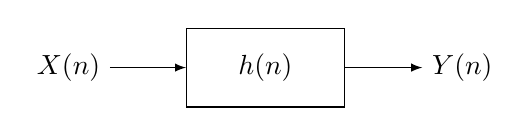
\begin{tikzpicture}[
    auto, 
    node distance=2cm,
    block/.style={rectangle, draw, minimum height=1cm, minimum width=2cm},
    >=latex
]
% Elemente des linearen Systems
\node at (0,0) (input) {$X(n)$};
\node[block] at (2.5,0) (system) {$h(n)$};
\node at (5,0) (output) {$Y(n)$};

% Verbindungspfeile
\draw[->] (input) -- (system);
\draw[->] (system) -- (output);
\end{tikzpicture}
\end{figure}

\FloatBarrier